\newpage
\section{Optimized GPU Implementation}
With regards to using SOA vs AOS: It makes sense to use SOA for this use case, because when we fill the shared memory, we only need to read the position and mass data of each body. A SOA layout allows us to read only those properties, without having to deal with the velocity data, which would otherwise be interleaved in an AOS layout. There might be a penalty for the update of the position, since the position data is stored separately from the velocity data, but this will be negligible compared to the performance gain on the force calculation.\\

We thus implemented the optimized version using a packed SOA data structure. We kept the Block Size constant at 128 for this and the following exercises, only varying the particle number. We used 1000 iterations for each simulation. \\
\begin{figure}[h]
    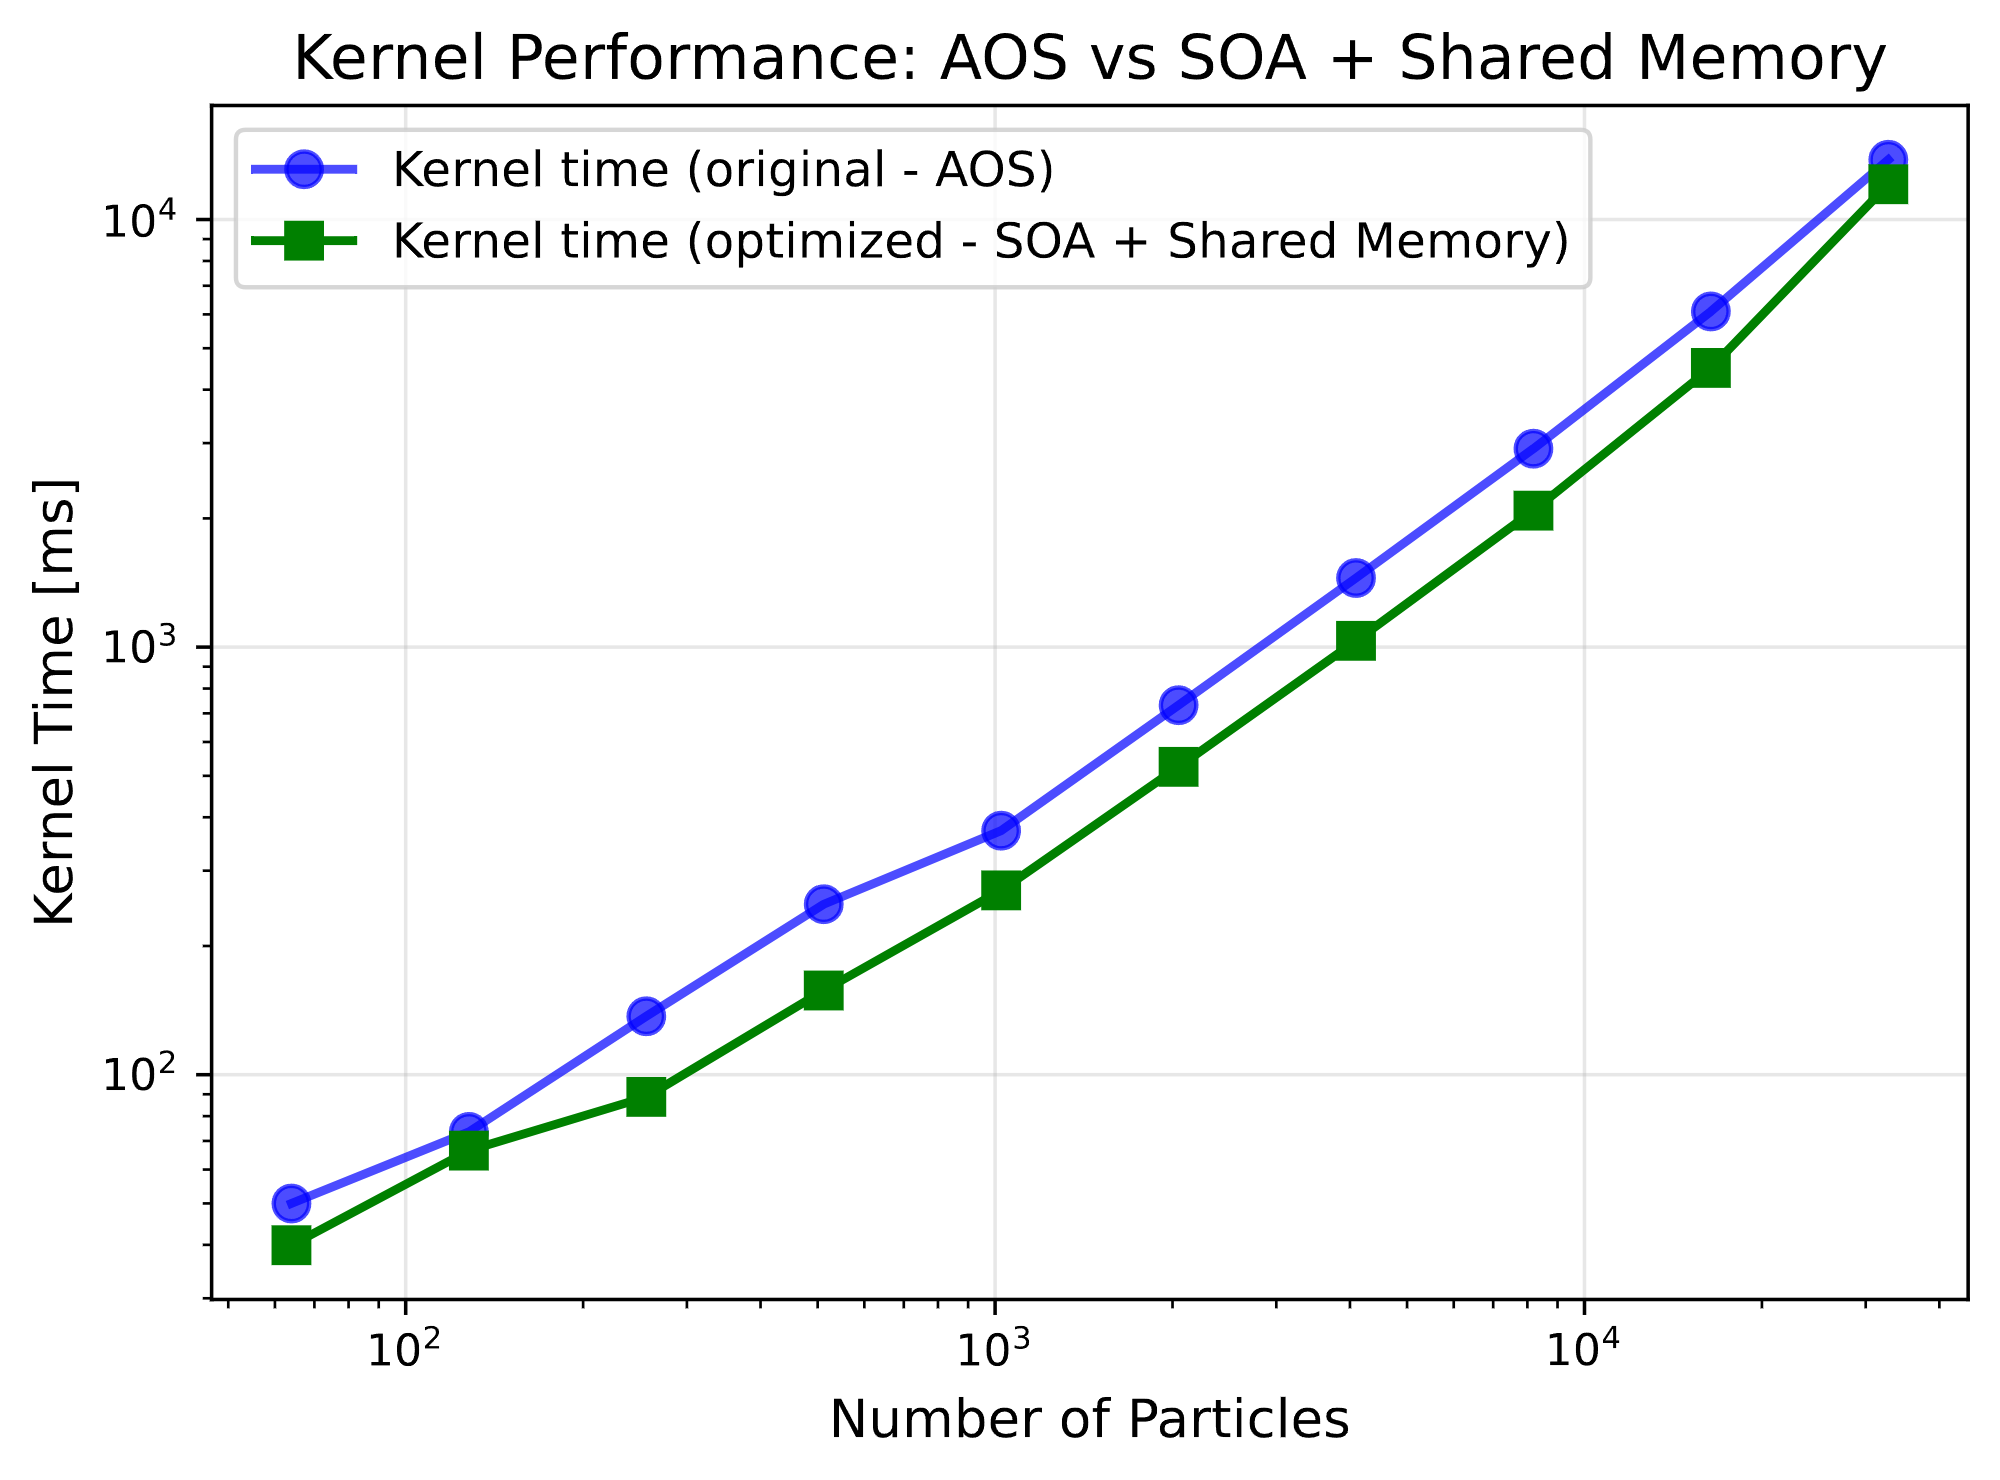
\includegraphics[width=1.0\textwidth]{Ex7_2_nbody_kernel_comparison.png}
    \caption{Kernel Performance: AOS vs SOA + Shared Memory}
    \label{fig:AOS_vs_SOA_SHARED}
\end{figure}
In this version (picture\ref{fig:AOS_vs_SOA_SHARED}) we also implemented tiling. This means we process small blocks of particles at a time, each one fitting into shared memory. We calculate the forces from this “source” block on all our “target” particles (one assigned to each thread) and then swap out for the next “source” block. The “source” blocks are always loaded into shared memory and shared between all threads in a block. Through this we can utilize the faster shared memory for our computations before moving on to the next block. We address global memory less, improving our speedup. \\

\begin{figure}[h]
    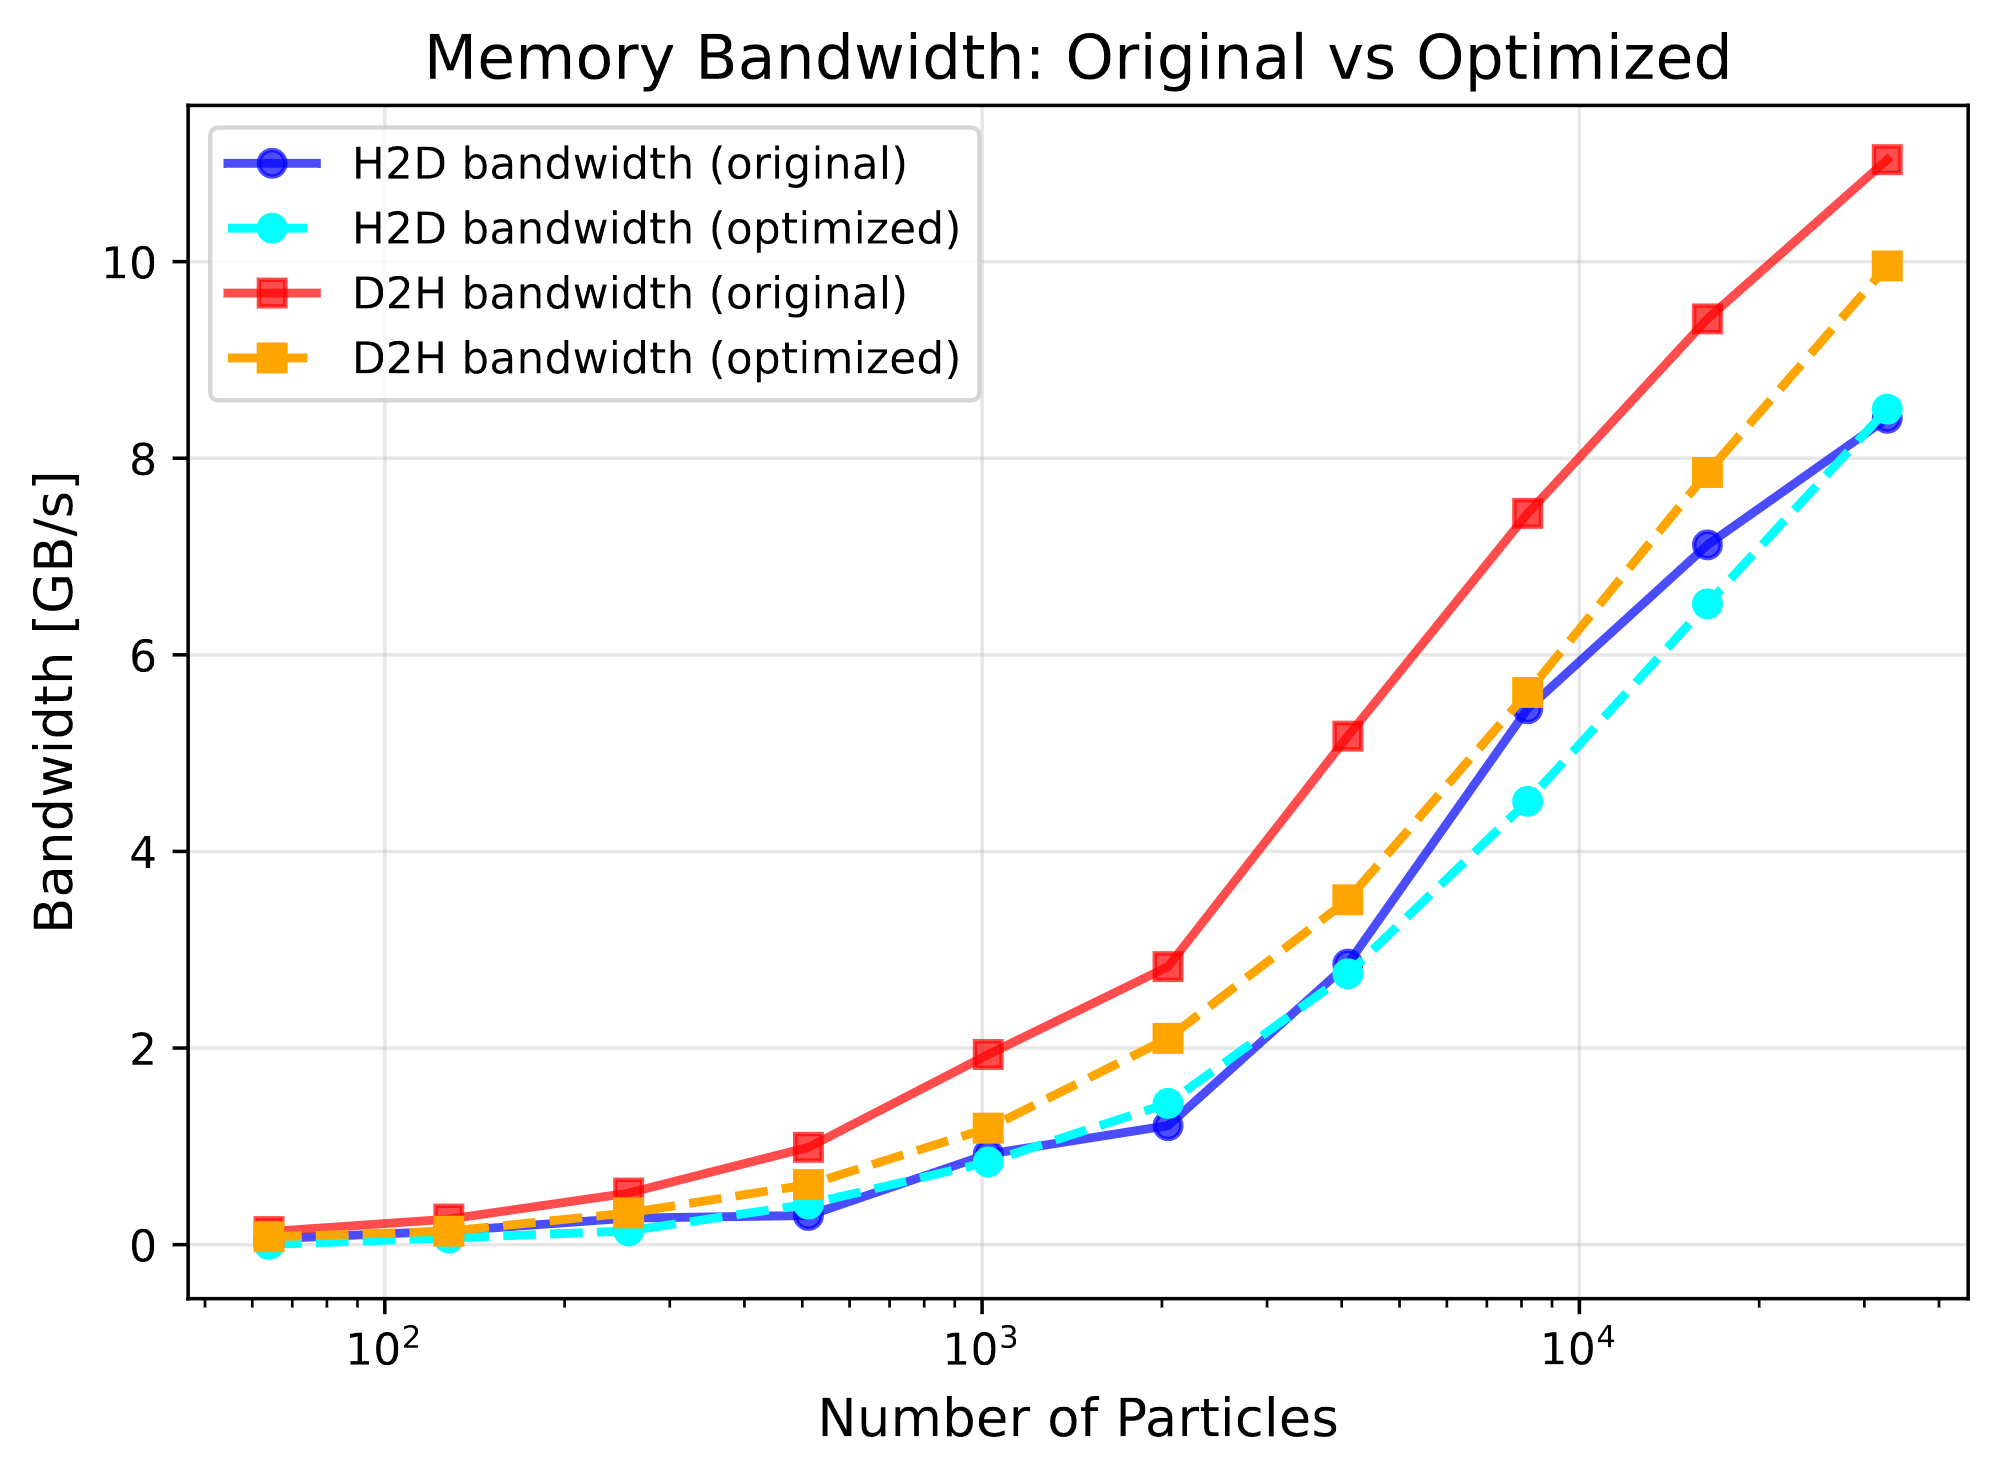
\includegraphics[width=1.0\textwidth]{Ex7_2_nbody_bandwidth_comparison.png}
    \caption{Memory Bandwidth: Original vs Optimized}
    \label{fig:Bandwidth_Comparision}
\end{figure}

Using both these optimizations we see a improvement in the kernel time, which is the most significant component of the total execution time, dominating both the d2h and h2d times (these are largely unaffected by the optimization, as no changes were made (picture \ref{fig:Bandwidth_Comparision})). We reach a maximum speedup of 1.59x against the benchmark and an average improvement of 1.35x over the particle numbers we tested. \\

\begin{figure}[h]
    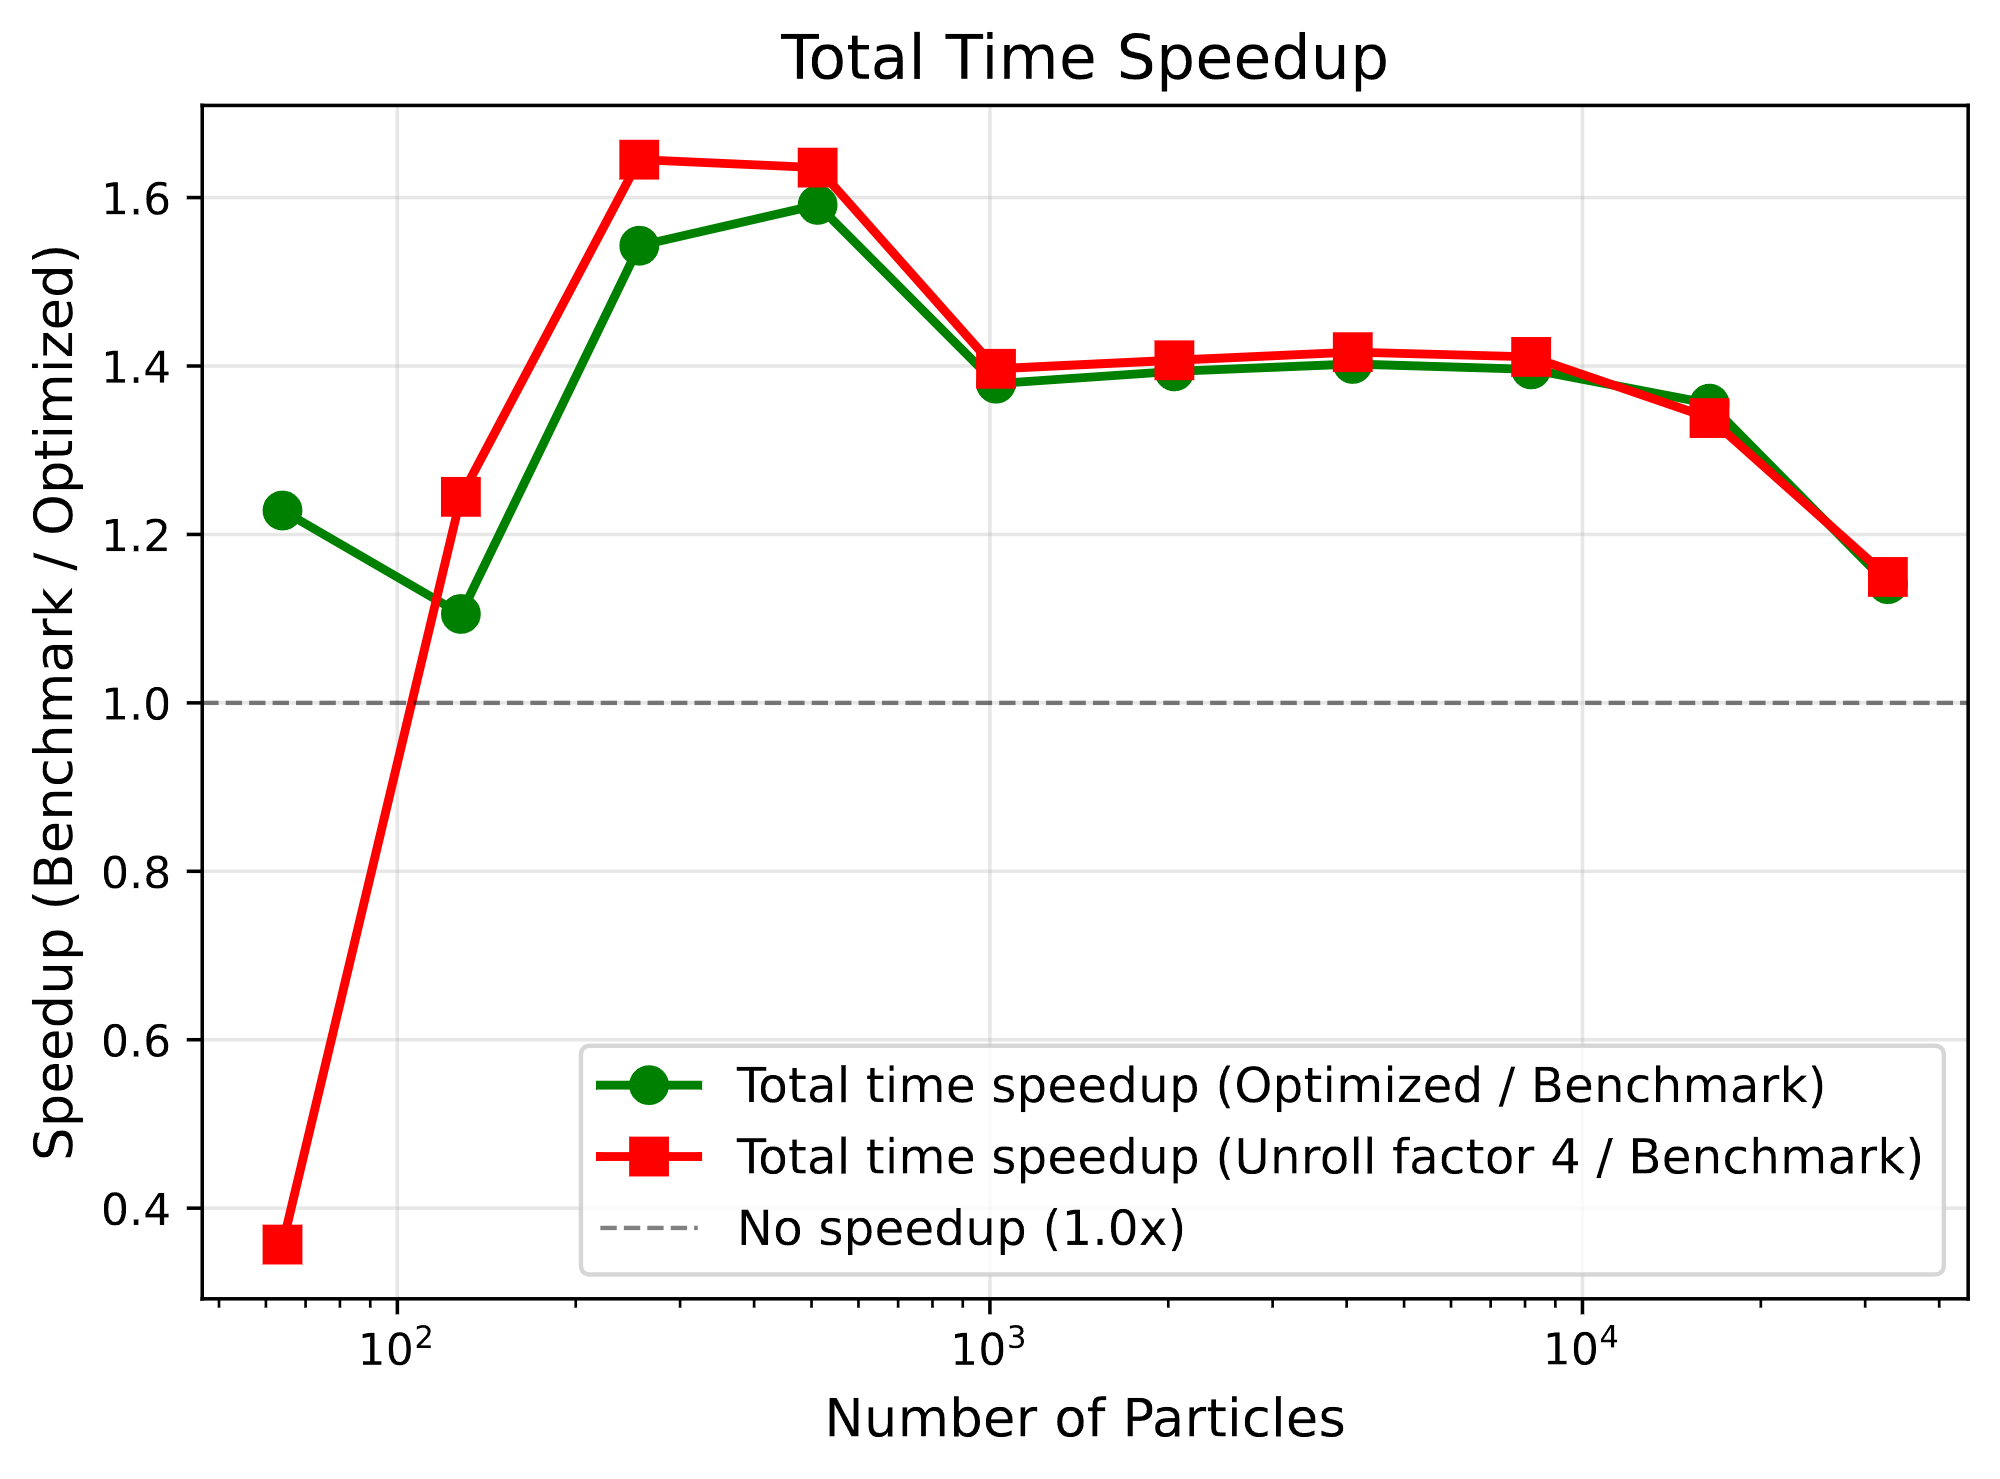
\includegraphics[width=1.0\textwidth]{Ex7_2_nbody_total_time_speedup.png}
    \caption{Speedup in Optimized and Uroll factor 4}
    \label{fig:Speedup_Optimized}
\end{figure}

Using loop unrolling within our kernels can further increases our performance, but only slightly. This is because the loops can already be pre-processed at compile time and thus can reduce overhead during runtime. It can however, also lead to a decrease in performance due to higher register pressure and increased code size. Using loop unrolling we increase our maximum speedup to 1.64x (picture \ref{fig:Speedup_Optimized}) over the benchmark, but decrease our average to 1.30x. How effective loop unrolling is, seems therefore to depend on the particle number.